\chapter{Grammar of Graphics Tools}
The Grammar of Graphics by Leland Wilkinson is a framework that provides a unique foundation for producing almost every quantitative graphic found in scientific journals, newspapers, statistical packages, and data visualization systems.

\section*{The Layers: An Overview}
\begin{minipage}[t]{0.6\textwidth}
    \vspace{0pt}
    The Grammar of Graphics follows a layered approach to describe and construct visualizations or graphics. 
    It provides a common language for thinking about the ways that design choices are made in visualization, describing everything from the data used to the visual channels displayed on the marks, and how data is converted into those channels.
    \hspace{1cm}
\end{minipage}
\begin{minipage}[t]{0.4\textwidth}
    \vspace{0pt}
    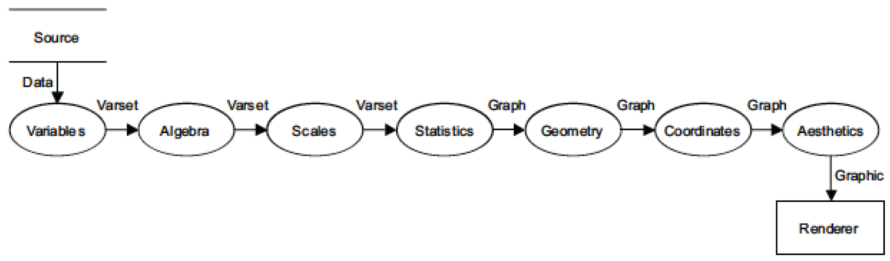
\includegraphics[width=\textwidth]{figures/grammar_flow.png}
    \captionof{figure}{Grammar of Graphics Flow \cite{wilkinsonHowMakePie2005}}
\end{minipage}
\captionsetup{justification=centering}

\vspace{-3mm}

\subsection*{Data}
\vspace{-2mm}
\begin{minipage}[t]{0.7\textwidth}
    In the first step, as described above, we aggregate and transform the data into a format we can later use to visualize and 
    perform further visual modifications on. 
    If we visualize the data at this step, we can see that the plot doesn't show much meaningful information yet.
    \hspace{1cm}
\end{minipage}
\begin{minipage}[t]{0.3\textwidth}
    \vspace{-20pt}
    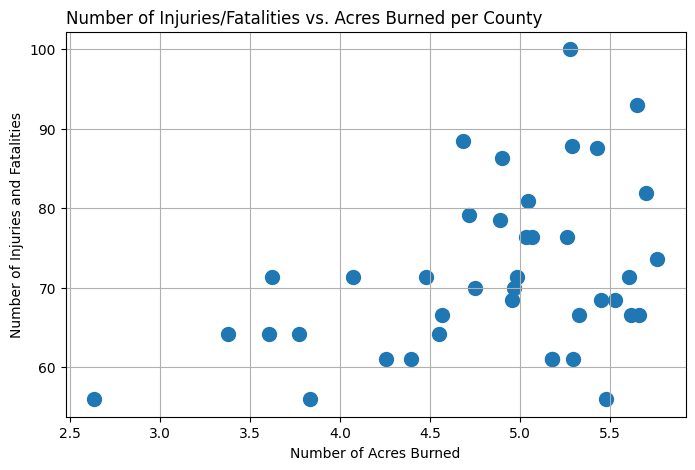
\includegraphics[width=\textwidth]{figures/gog_data.png}
    \captionof{figure}{Grammar of Graphics: Data}
\end{minipage}


\vspace{-3mm}

\subsection*{Aesthetics}
\vspace{-2mm}
\begin{minipage}[t]{0.7\textwidth}
    In the Grammar of Graphics, the Aestehetics Layer refers to the mapping of one or more variables to one or more visual elements on the graph. This includes 
    mapping variables to the x-axis, y-axis, and using color to differentiate different attributes. Aesthetics are essential in creating meaningful and 
    effective visualizations \cite{wilkinsonAesthetics2005}.
    In this example we map the \texttt{AcresBurned} variable to the x-axis and the sum of \texttt{Injuries} and \texttt{Fatalities} variables to the y-axis. Additionally,
    the Admin Units (fire departments) get added as a third dimension by using color.
    \hspace{1cm}
\end{minipage}
\begin{minipage}[t]{0.3\textwidth}
    \vspace{-20pt}
    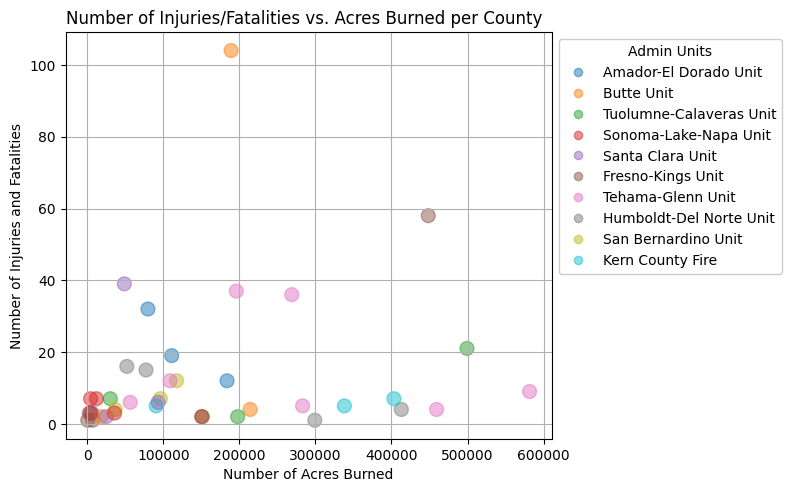
\includegraphics[width=\textwidth]{figures/gog_aesthetics.png}
    \captionof{figure}{Grammar of Graphics: Aesthetics}
\end{minipage}

\vspace{-3mm}

\subsection*{Scale}
\vspace{-2mm}
\begin{minipage}[t]{0.7\textwidth}
    In the Grammar of Graphics, the Scale step can include the scaling of the data, but 
    also the scaling of the visual elements, such as the axes or scatter sizes \cite{wilkinsonScales2005}.
    In this example we added another dimension to the plot by utilizing the scale of scatters (Fire Dept. Size) 
    to visualize the number personnel that was involved. Additionally, since most of the scatters were overlapping
    in the previous linear x-scale, we switched to a logarithmic scale for the x-axis.
    \hspace{1cm}
\end{minipage}%
\begin{minipage}[t]{0.3\textwidth}
    \vspace{-20pt}
    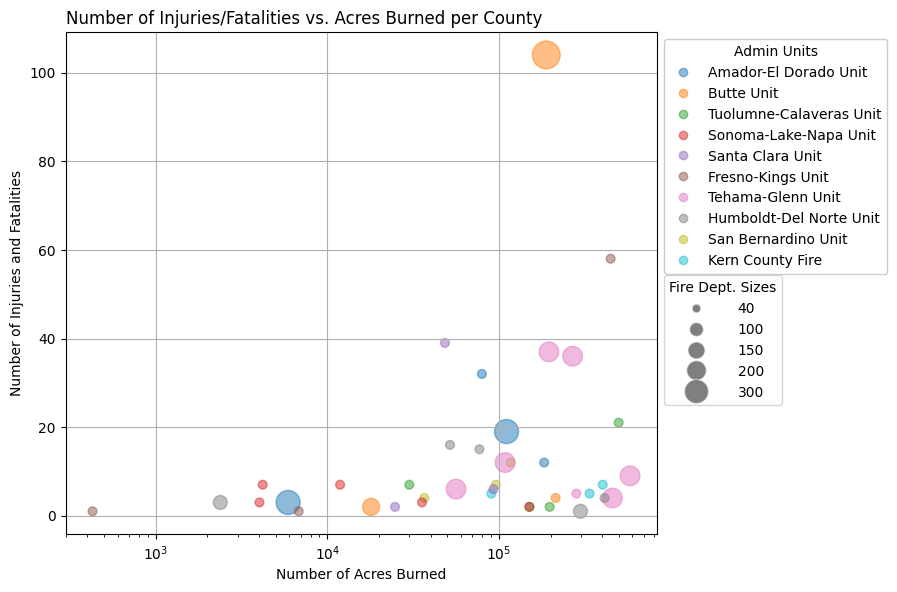
\includegraphics[width=\textwidth]{figures/gog_scale.png}
    \captionof{figure}{Grammar of Graphics: Scale}
\end{minipage}

\vspace{-2mm}

\subsection*{Geometry}
\vspace{-2mm}
\begin{minipage}[t]{0.6\textwidth}
    We can use the Geometry Layer of the Grammar of Graphics to access further dimensions without having to
    add more axes in the sense of a 3D plot \cite{wilkinsonGeometry2005}. In this example we use the shape-property of the scatterplot and
    its scatters to visualize the fuel types that accelerated a wildfire. As each scatter represents a county
    the shape of the scatter describes the county's major fuel type; The type of fuel that is responsible the most
    in a given county.
    \hspace{1cm}
\end{minipage}%
\begin{minipage}[t]{0.4\textwidth}
    \vspace{-20pt}
    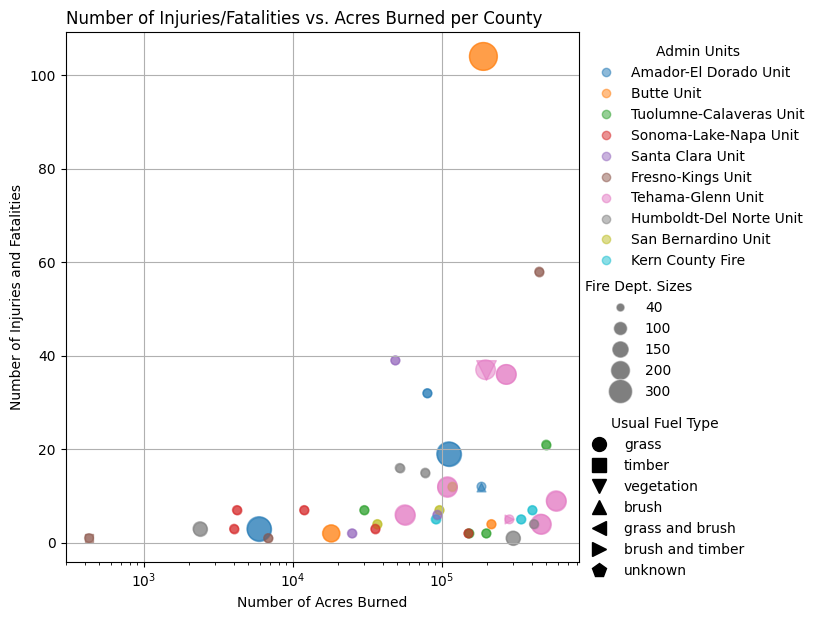
\includegraphics[width=\textwidth]{figures/gog_geometry.png}
    \captionof{figure}{Grammar of Graphics: Geometry}
\end{minipage}

\vspace{-2mm}

\subsection*{Statistics}
\vspace{-2mm}
\begin{minipage}[t]{0.6\textwidth}
    Showing statistical features in a visualization helps the viewer to form a better
    contextual understanding as for example the mean provides a good reference point for
    an ``Expected Value'' or the general center of data with the intersection of the \texttt{vline} and \texttt{hline} \cite{wilkinsonStatistics2005}.
    
    In other types of  options include to show a confidence interval or a regression line.
    \hspace{1cm}
\end{minipage}%
\begin{minipage}[t]{0.4\textwidth}
    \vspace{-20pt}
    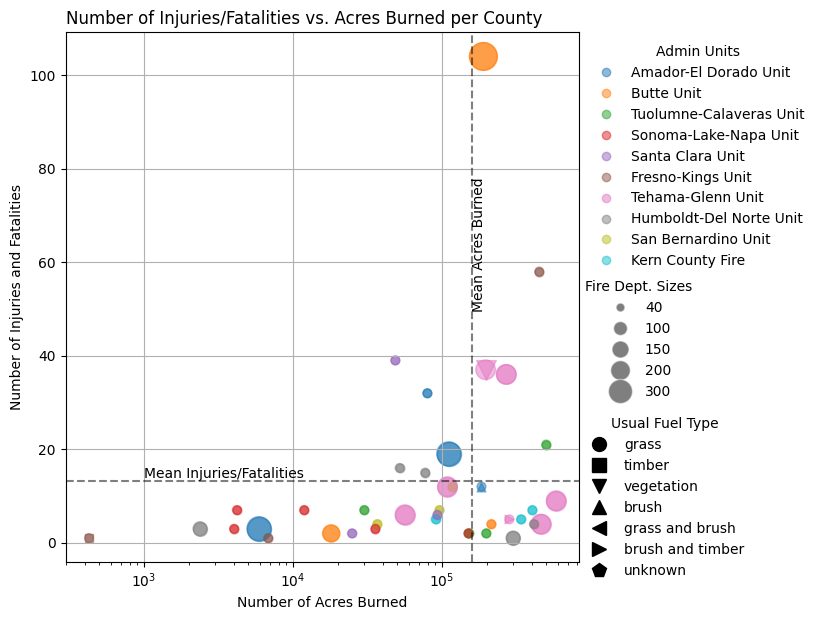
\includegraphics[width=\textwidth]{figures/gog_statistics.png}
    \captionof{figure}{Grammar of Graphics: Statistics}
\end{minipage}

\vspace{-2mm}

\subsection*{Facets}
\vspace{-2mm}
\begin{minipage}[t]{0.6\textwidth}
    Facets in the Grammar of Graphics are a way to split data into subplots based on another factor 
    in the data. They allow for the creation of multiple small multiples, each showing a 
    different subset of the data.
    In this case, the plot we are working on was split into five subplots, one for each category of fire department size.
    The respective Admin Unit (fire dept.) of each county has a size which represents how many personnel were involved 
    in the fire.
    \hspace{1cm}
\end{minipage}%
\begin{minipage}[t]{0.4\textwidth}
    \vspace{-20pt}
    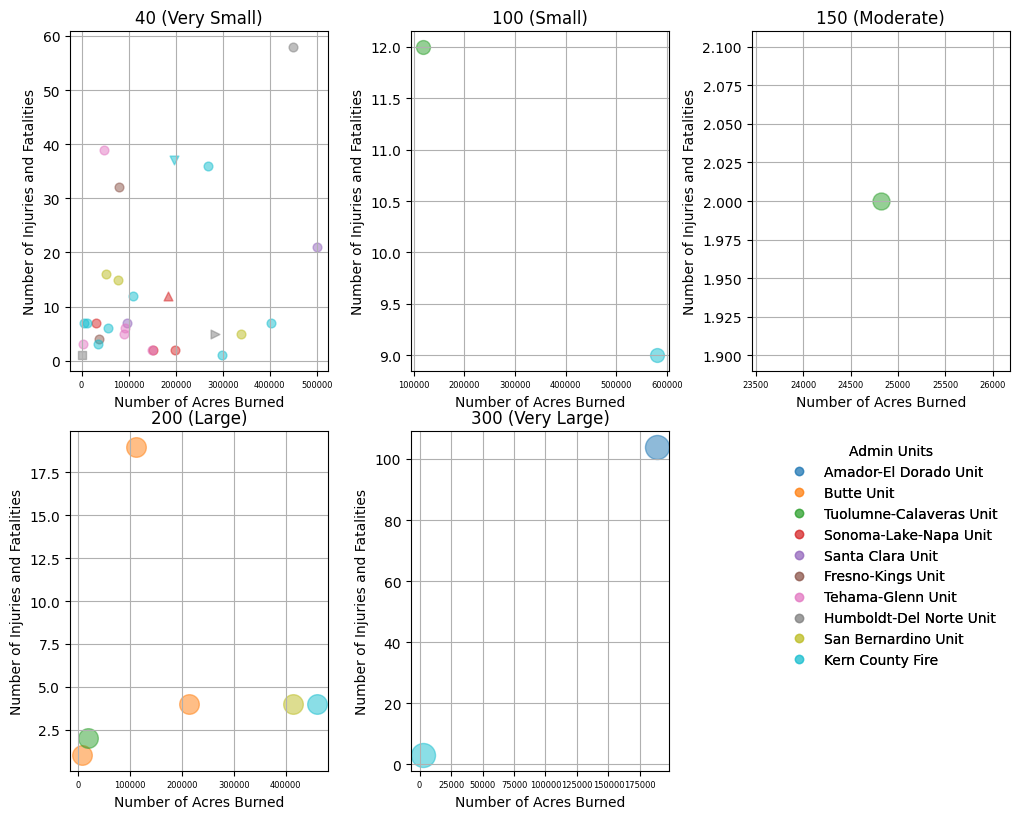
\includegraphics[width=\textwidth]{figures/gog_facets.png}
    \captionof{figure}{Grammar of Graphics: Facets}
\end{minipage}

\vspace{-2mm}

\subsection*{Coordinates}
\vspace{-2mm}
When looking at coordinates in the context of the Grammar of Graphics, we are referring to 
the coordinate system of the plot \cite{wilkinsonCoordinates2005}. This includes the type of coordinate system, such as Cartesian 
or Polar. It also includes the range of the coordinate system, such as the range of the x-axis and y-axis.

In this case, we have implemented a Cartesian coordinate system with a logarithmic x-axis. 
Choosing what kind of coordinate system to use mainly depends on the type of the underlying data.
The most common coordinate system is the Cartesian coordinate system as it is very intuitive for 
human perception. Polar coordinates on the other hand are hard to comprehend as humans usually perform
rather bad when it comes to interpreting angles, which is the main component of polar coordinates \cite[Chapter~7]{alma99116746755205518}.